%! Author = shenyixiao
%! Date = 13/03/2023
%%%%%%%%%%%%%%%%%%%%%%%%%%%%%%%%%%%%%%%%%%%%%%%%%%%%%%%%%%%%%%%%%%%%%%%%%%%%%%%%%%%%%%%%%%%%%%
%Packages
%%%%%%%%%%%%%%%%%%%%%%%%%%%%%%%%%%%%%%%%%%%%%%%%%%%%%%%%%%%%%%%%%%
\documentclass[12pt, a4paper]{report}
\usepackage{graphicx, listings, framed, mdframed, float}
\usepackage{appendix, pdfpages, setspace, color, hyperref}
\usepackage{tocloft}                    % This squashes the Table of Contents a bit
\hypersetup{colorlinks=true}            % To avoid the borders around hyperlinks
\hypersetup{colorlinks, citecolor=black, filecolor=black, linkcolor=black, urlcolor=black}
\definecolor{MyLightYellow}{cmyk}{0,0.,0.2,0} % Used for program listings
\definecolor{shadecolor}{cmyk}{0,0.2,0,0} % Used for snugshade listings
\usepackage[top=3cm, bottom=3cm]{geometry}
\usepackage{listings}
\usepackage{subcaption}
\usepackage{xcolor}
\setlength{\parskip}{10pt}                % sets spacing between paragraphs
\interfootnotelinepenalty=500             % this prevents footnotes breaking across pages
%%%%%%%%%%%%%%%%%%%%%%%%%%%%%%%%%%%%%%%%%%%%%%%%%%%%%%%%%%%%%%%%%%%%%%%%%%%%%%%%%%%%%%%%%%%%%%
%Commands
%%%%%%%%%%%%%%%%%%%%%%%%%%%%%%%%%%%%%%%%%%%%%%%%%%%%%%%%%%%%%%%%%%
\renewcommand\bibname{References}         % to change Bibliography to References
\renewcommand\lstlistlistingname{List of Code Listings}
\newcommand{\HRule}{\rule{\linewidth}{0.75mm}} % needed on title page

%%%%%%%%%%%%%%%%%%%%%%%%%%%%%%%%%%%%%%%%%%%%%%%%%%%%%%%%%%%%%%%%%%%%%%%%%%%%%%%%%%%%%%%%%%%%%%
%document
%%%%%%%%%%%%%%%%%%%%%%%%%%%%%%%%%%%%%%%%%%%%%%%%%%%%%%%%%%%%%%%%%%
\begin{document}



\begin{center}
	\includegraphics[width=0.4\textwidth]{fileForWriting/BigCrest}\\ \vspace{15 mm}
	\textsc{\Large Year 2 Project}\\ \vspace{15 mm}
	\doublespace
	\HRule \\ \vspace{8 mm}
	{\huge \bfseries Wearable Sensor}       % <<<< Put your title here
	\\\vspace{4 mm}
	\HRule \\ \vspace{25 mm}

	Name \textsc{Surname1} (ID 2054321)      \\        % <<<< Your names
	Name \textsc{Surname2} (ID 2052234)      \\        % <<<< Your names
	Name \textsc{Surname2} (ID 2052234)      \\        % <<<< Your names
	Name \textsc{Surname2} (ID 2052234)      \\        % <<<< Your names
	Name \textsc{Surname2} (ID 2052234)      \\        % <<<< Your names
	Group 2p23                                 \\        % <<<< Your group number

	\vspace{15mm}
	\emph{Supervised by } Dr Name \textsc{Surname}     % <<<< Your supervisor
	\vfill             % Bottom of the page
	{\large \today}    % today's date
\end{center}

%%%%%%%%%%%%%%%%%%%%%%%%%%%%%%%%%%%%%%%%%%%%%%%%%%%%%%%%%%%%%%%%%%%%%%%%%%%%%%%%%%%%%%%%%%%%%%
%Abstract
%%%%%%%%%%%%%%%%%%%%%%%%%%%%%%%%%%%%%%%%%%%%%%%%%%%%%%%%%%%%%%%%%%
\begin{abstract}
	This document serves as a template to show you how to present and structure your project dissertation. In the interests of uniformity of format, you are asked not to significantly alter the format and layout of this \LaTeX~ document. The chapter names and structure are intended as a guide, and you are welcome to change these as appropriate. While this is not a definitive guide to dissertation writing, it is intended as a guide to assist in documenting and presenting your project work in an academic and professional manner, and reflects the expectations of those in academia and industry who are likely to read your report. Appended to this guide are some real examples of common mistakes that should be avoided.

	Your Abstract is expected to be between 100 and 250 words in length, and should summarise the problem, outline the approach adopted, and summarise the project findings or results. It's the first (and possibly the only) part to be read, and should provide a snapshot of the whole project in 2 or 3 paragraphs.
\end{abstract}



%%%%%%%%%%%%%%%%%%%%%%%%%%%%%%%%%%%%%%%%%%%%%%%%%%%%%%%%%%%%%%%%%%%%%%%%%%%%%%%%%%%%%%%%%%%%%%
%Declaration
%%%%%%%%%%%%%%%%%%%%%%%%%%%%%%%%%%%%%%%%%%%%%%%%%%%%%%%%%%%%%%%%%%
\newpage
\rule{0mm}{30mm}
\centerline{\textbf{Declaration}}

\fbox{\parbox{0.92\textwidth}{I confirm that I have read and understood the University’s definitions of plagiarism and collusion from the Code of Practice on Assessment. I confirm that I have neither committed plagiarism in the completion of this work nor have I colluded with any other party in the preparation and production of this work. The work presented here is my own and in my own words except where I have clearly indicated and acknowledged that I have quoted or used figures from published or unpublished sources (including the web). I understand the consequences of engaging in plagiarism and collusion as described in the Code of Practice on Assessment (Appendix L).}}



%%%%%%%%%%%%%%%%%%%%%%%%%%%%%%%%%%%%%%%%%%%%%%%%%%%%%%%%%%%%%%%%%%%%%%%%%%%%%%%%%%%%%%%%%%%%%%
%Contents
%%%%%%%%%%%%%%%%%%%%%%%%%%%%%%%%%%%%%%%%%%%%%%%%%%%%%%%%%%%%%%%%%%
\newpage \tableofcontents
\newpage \listoffigures
\newpage \listoftables
\newpage \lstlistoflistings        % this is for program listings; if you don't have any, remove this line

\newpage \onehalfspace   %containging titlepage & abstract & declaration & table of contents...
\chapter{Introduction}
Avian flight dynamics have been a topic of interest for many researchers over the years.
In order to study the indoor wingbeat action of birds, previous research has utilized optical motion capture systems.
\cite{ju_data-driven_2011}
    \textcolor{red}{NEED ONE REFERENCE HERE.} %todo: zoology studies using optical bio-logging systems. (ju_data-driven_2011)
While such optical bio-logging systems have been helpful in collecting data for analysis and simulation, they are limited by site constraints and high costs.

Recent studies have attempted to address these limitations by installing single inertial measurement unit (IMU) on birds to acquire basic wingbeat data.
%todo: zoology studies using non-optical bio-logging systems, often with single type of sensors. (lissaman_wind_2005, taylor_birds_2019, gomez_laich_identification_2009)
\textcolor{red}{NEED THREE REFERENCE HERE}.
However, the data collected from a single IMU is narrowed and does not capture the complete wingbeat action of birds. There is still a significant research gap in the development of a multi-IMU bio-logging device capable of comprehensively capturing the entire wingbeat action of birds.

To fill such research gap, this project aims to design a simple wearable sensor system based on four IMUs for human walking pattern recognition, capturing comprehensive motion data that can be used for analysis and simulation purposes. Furthermore, a front-end display engine utilizing an external JavaScript graphic library will also be created to quickly generate a digital twin of humans. This will not only enable motion tracking capabilities, but also allow for easy monitoring through a web browser with rapid deployment.

While the initial testing of the technology will be conducted on human subjects, the potential applicability of this technology in tracking the movement and behavior of birds is promising. The data collected by this device provides a valuable opportunity to gain insights from the intricate and sophisticated designs found in nature. For instance, one potential application is to study the flight patterns of birds and how they utilize their wings to achieve optimal efficiency, especially when faced with varying wind directions.

In conclusion, this research project aims to fill the research gap in the development of a multi-IMU bio-logging device capable of comprehensively capturing a complete motion of objects. The proposed device has the potential to contribute not only to the research on avian flight dynamics but also to the field of zoology more broadly. Simultaneously, such device will be designed to be simple, cost-effective, and easy-using, providing a useful tool for researchers in various fields.


%Nonetheless, a significant research gap remains in the development of a multi-IMU bio-logging device capable of comprehensively capturing the complete wingbeat motion of birds without any space limitations.
%todo: future improvement, existed non-optical bio-logging systems---> machine learning ---> process data in depth


\section{Objectives}
    The main objective of this project is to develop a digital representation of a human using wearable sensors.
    To accomplish this objective, the following three sub-objectives have been outlined:
\begin{enumerate}\label{obj}
    \item \label{itm:obj-data-collection}Data collection:
    Design a wearable device capable of collecting lower body motion data by attaching four IMUs, two on each femur and tibia.
    To enable unrestricted movement without the need for cables, the device will feature wireless communication capabilities.
    In addition, the device will integrate an independent power source to ensure uninterrupted data collection during testing.

    \item \label{itm:obj-data-integration}Data integration:
    A simple C++ socket server will be developed to serve as the central hub for collecting and processing the motion data collected by the IMUs.
    This server will also be responsible for transmitting files to the front-end.

    \item \label{itm:obj-model-creation} Model creation:
    To enable the core functionality of motion-following, a simple front-end displaying engine will be developed to create a model of the human body.
    This model will be generated using the motion data collected by the IMUs and will serve as the basis for further analysis and research.
\end{enumerate}


  %containging backgrounds...
\chapter{Design and Implementation}

\section{Architecture design}

%-----------This is a FIGURE-----------------------
\begin{figure}[htbp]
	\centering
	\includegraphics[clip, trim=0cm 0cm 0cm 0cm, width=1\textwidth]{
		fileForWriting/sketch_map}
	\caption[Project architecture diagram]{Project architecture diagram. }
	\label{fig:project-architecture-diagram}
\end{figure}
%--------End of this FIGURE -----------  

In order to ensure efficient task allocation, the project was partitioned into two modules as Figure~\ref{fig:project-architecture-diagram} has shown: hardware and software.
The hardware system was delegated to three MRS students, based on their respective areas of expertise and preferences.
Their responsibilities encompassed the utilization of Arduino to collect data from multiple sensors through an inter-integrated circuit (IIC, or I2C) multiplexer, and an implementation of wireless transmission.
Additionally, a backup plan utilizing wired communication through USART was selected, considering the development timeline and difficulty of using a Wi-Fi module.

On the other hand, the software module was entrusted to two CSEE students.
The responsibilities of the two CSEE students encompassed two tasks.
The first one is to construct a simple C\texttt{++} socket server to function as the data center.
Secondly, they were tasked with developing a rudimentary human lower limb model using three.js, an external JavaScript graphic library~\cite{threejs}.

Upon achieving these objectives, users would be able to access the visualized digital twin directly through a web browser with ease.
To facilitate debugging, the entire network would operate within a local area network (LAN). However, it could be expanded to the Internet in the future.

\section{Real-time rendering design}
%-----------This is a FIGURE-----------------------
\begin{figure}[htbp]
	\centering
	\includegraphics[clip, trim=0cm 0cm 0cm 0cm, width=\textwidth]{
		fileForWriting/sequence}
	\caption[Transmitting logic of motion data]{Transmitting logic of motion data collected by IMUs, where a single pose represents data from four IMUs, two each from the femur and tibia.}
	\label{fig:sequence}
\end{figure}
%--------End of this FIGURE -----------
In this project, real-time rendering is designated as a potentially critical task metric.
To achieve such functionality, two key steps are thus implemented.
The first step is to ensure that the front-end could access the latest motion data.
On the server, a thread is dedicated to continuously writing motion data from the IMU to the same text file.
As the left hand side of Data-displaying loop in Figure~\ref{fig:sequence} may illustrate, once the front-end browser request a pose data, another thread of server will be launched to read the last line of the txt file and send it back to the client.

The second operation aims to reduce the latency in wireless communication .
In the displaying engine, a method of multi-threading is employed.
Specifically, one thread is designed to only render the animation, while another one is responsible for requesting data from the server and interpolating the returned data for use in the next rendering.
This approach may not only smooth the animation but also offset some latency raised in the wireless communication.

\section{3D model design}

%-----------This is a FIGURE-----------------------
\begin{figure}[htbp]
	\centering
	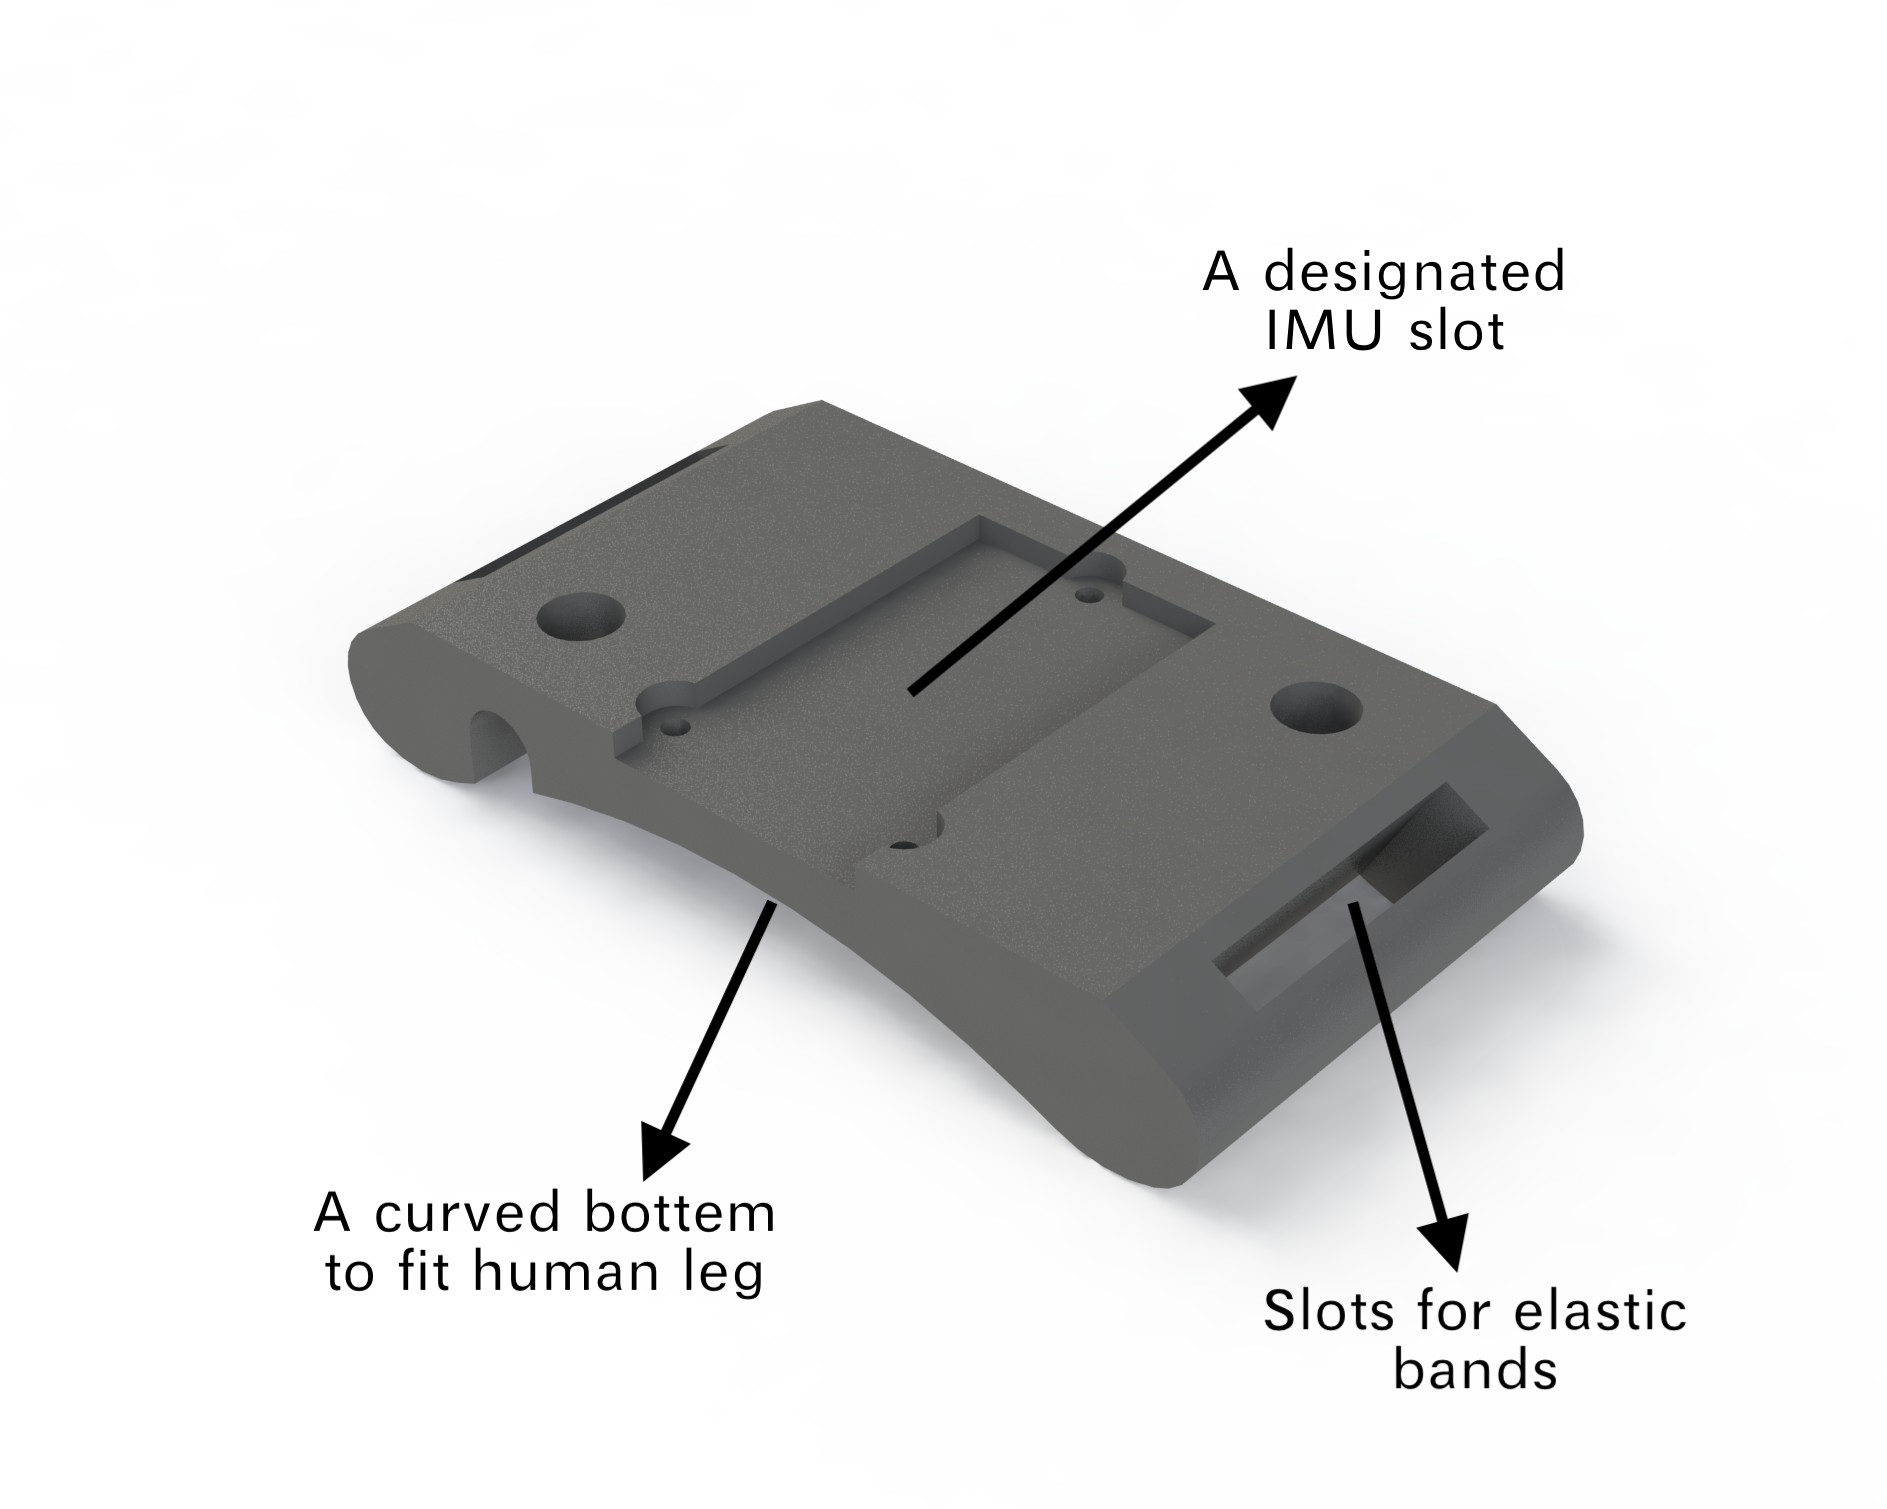
\includegraphics[width=\textwidth]{
		fileForWriting/3d-model}
	\caption[Model for holding an IMU on the femur]{Model for holding an IMU on the femur (rendered by SolidWorks Software).}
	\label{fig:3d-model}
\end{figure}
%--------End of this FIGURE -----------  


The IMU-holding component for the femur and tibia has been designed with a flat top edge and a curved bottom edge, as shown in Figure~\ref{fig:3d-model}.
It conforms precisely to the curve of the human leg, resulting in a more comfortable fit.
To minimize shock and vibration to IMU during testing, a form tape has been added into the designated IMU slot.
Additionally, adjustable VELCRO straps have been incorporated into the component to accommodate different leg sizes, ensuring ease and speed of use.

Furthermore, two protective techniques have been applied for preventing damage to the data cable during testing.
Firstly, a spiral wrap has been added to the data cable to provide additional protection.
Finally, each component has been perforated with holes, through which a hemp rope will be threaded to prevent external forces from dislodging the cable.
 %architecture design
\chapter{Materials and Methods}


\section{Materials}


\subsection{Main component list}
\begin{enumerate}
	\item   Arduino-UNO-Wifi-Rev2: an upgraded version of the standard Arduino UNO board that incorporates several additional features to enhance its functionality.
	In this project, the onboard Wi-Fi module was fully used to provide a wireless communication.
	\item   Grove IMU 9DOF (ICM20600+AK09918): an inertial measurement unit module that integrates three sensors, including an accelerometer, gyroscope, and magnetometer.
	However, this module does not have a physical circuit of temperature compensation.
	Additionally, the chip ICM20600 only supports configuring two kinds of IIC addresses.
	Relevant datasheet is shown in Figure~\ref{fig:limited-IIC-address} in Appendix.
	\item   Gravity IIC Multiplexer: a powerful module that allows for the expansion of the IIC bus on Arduino.
	It solves the problem of overlapping IIC address.
	\item   Multi-core screened cable: to ensure the quality of wired communication.
	\item   TP-Link AC1200 Wireless Dual Band Router: to provide a local area network.
	\item   18650 2,600mAh Lithium Rechargeable Batteries: a built-in power source.
	\item   Velcro Brand Adjustable Straps, 25mm x 680mm.
\end{enumerate}


\subsection{Software}
\begin{enumerate}
	\item JetBrains CLion: for socket server programming;
	\item Arduino IDE \& PlatformIO: for Arduino programming;
	\item Autodesk Fusion 360 \& SolidWorks \& SketchUp: for creating 3D models;
	\item Three.js: for front-end programming;
\end{enumerate}


\section{Methods}


\subsection{Arduino: data collection}\label{subsec:data-fetching}
\begin{enumerate}
	\item   Firstly, connect the IIC multiplexer's VCC, GND, SDA, and SCL pins to the respective pins on the Arduino.
	All the cables used were initially of the GROVE type, which were later replaced by screened cables.
	\item   Then, each IMU was connected to one of the IIC multiplexer channels.
	The port setting was saved into the code as portrayed in List~\ref{lst:port-saving}.

	\lstset{language=C++}
	\begin{lstlisting}[caption=Saving the port setting of four IMUs.,    numbers=left,
		firstnumber=22, label={lst:port-saving}]
//port number
enum portConfiguration {
    IMU_LEFT_FEMUR = 2,
    IMU_RIGHT_FEMUR = 6,
    IMU_LEFT_TIBIA = 5,
    IMU_RIGHT_TIBIA = 7
};
	\end{lstlisting}

	\item   After that, install relevant libraries to drive the hardware components, such as the ``IMU-ICM20600.h'' for IMU and ``DFRobot\_I2C\_Multiplexer.h'' for multiplexer.
	Due to some reading issues encountered while using the magnetic sensor, the current project only utilized a 6DOF transformation.
	The initialization logic of four IMUs is shown below, where the default data rate for IMU was set to be 100 Hz.

	\lstset{language=C++}
	\begin{lstlisting}[    numbers=left,
		firstnumber=30, caption=Inilizing the multiplexer as well as four IMUs,label={lst:hardware-init}]
I2CMulti.begin();   //init the multiplexer
for (int i = 0; i < 8; i++) {
    if (i == IMU_LEFT_FEMUR
        || i == IMU_RIGHT_FEMUR
        || i == IMU_LEFT_TIBIA
        || i == IMU_RIGHT_TIBIA) {
        I2CMulti.selectPort(i);
        IMU_external.initialize();  //init the IMU
        IMU_external_data[i].filter.begin(100);
        delay(100);
    }
}
	\end{lstlisting}

	\item   After initialization, a calibration process was followed to improve the accuracy and reliability of the measurements.
	It was achieved by averaging the output data in the first three seconds where the IMUs were motionless.
	Then, future output would be reduced by this average to reduce factors of potential manufacturing variations or sensor drift.
	Relevant code is included in List~\ref{lst:init-arduino} in Appendix.

	\item   To obtain the motion data, the attitude and heading reference system (AHRS) library named Mahony was utilized to generate Euler angles from raw data.
	It is a set of algorithms designed to estimate the attitude and orientation of objects in three-dimensional space using fusion algorithms such as Kalman filter, Madgwick filter, and Mahony filter.
	These tools enable fusing the raw data of IMUs to obtain more accurate, stable, and reliable attitude information.
	The Mahony library, which is a popular sensor fusion algorithm, was selected for the experiment due to its higher computational efficiency.
	Additionally, it contains a 6DOF transformation without using magnetic sensors.

\end{enumerate}


\subsection{Arduino: wireless communication} \label{subsec:5g-network}
\begin{enumerate}
	\item   To enable the built-in Wi-Fi module on Arduino-UNO-Wifi-Rev2, an external library called WiFiNINA was chosen and implemented.
	This library, provided by the official Arduino website, facilitates communication between the microcontroller and the onboard wi-fi module through a serial peripheral interface (SPI).
	It also provides some simple examples for studying.
	\item   Initially, the Arduino was connected to a 2.4G network and attempted to establish a connection with a remote server through a handshake process.
	These functions are all included in the library and have been implemented in the kernel.
	\item   Next, a simple const string message was written to one Arduino's socket and later sent by kernel.
	Given that the server was capable of printing any incoming message, the message was finally displayed on the server's console as intended.
	\item   Following this, a stress test was conducted to evaluate the system's capacity to send a high volume of data.
	This was accomplished by continuously sending an increasing number to the server, which was then printed by the server.
	Meanwhile, the Arduino would also print out the message sent through a serial communication to the computer.
	By such comparison, the latency caused in this process could be roughly estimated.
\end{enumerate}


\subsection{Socket server}
\begin{enumerate}
	\item   Based on an example sketch from an online book~\cite{beej-guide}, a simple C\texttt{++} socket server was built to support responding basic HTTP-GET requests.
	\item   Additionally, a multi thread was added to asynchronously save the motion data sent from Arduino.
	\item   To enhance the transmission of motion data to front-end users, a custom JSON encoder was developed to package the raw motion data into a compact and efficient JSON format as List~\ref{lst:json} shows.
	To increase communication rate, the content in such format has been extremely reduced by using abbreviations, where ``L\_F'' represents the motion data of left femur.
	The Euler angles were also abbreviated to ``y'', ``r'', and ``p''.
	Relevant code of the JSON formatter is in List~\ref{lst:json-formatter} in Appendix.
\end{enumerate}

\lstset{
	language=json,
	numbers=left,
	firstnumber=1
}
\begin{lstlisting}[caption={JSON code sent to front-end client.},label={lst:json}]
{
	"L_F": [{
		"y": -0.01,
		"r": 1.82,
		"p": -0.52}],
	"R_F": [{
		...
}
\end{lstlisting}


\subsection{Displaying engine}\label{subsec:engine}

With the tutorial given by official three.js website~\cite{threejs}, a simple static 3D model generator was thus implemented.
However, such basic generator was not flexible enough to rapidly create a specific model, such as humans or birds.
Hence, a function that can generate models according to user customization was developed.
It works like a text operator and user could change his text to modify a corresponding model subsequently.
Relevant results are presented in the next chapter.
In the meantime, the following are the main implementation of this displaying engine:

%-----------This is a FIGURE-----------------------
\begin{figure}[htbp]
	\centering
	\includegraphics[width=0.5\textwidth]{
		fileForWriting/browser_sequence}
	\caption[Sequence diagram of the displaying engine]{Sequence diagram of the displaying engine.}
	\label{fig:browser_sequence}
\end{figure}
%--------End of this FIGURE -----------


\subsubsection{Reduce latency: multi-thread}
To fully achieve the goal of real time rendering, as depicted by the sequence diagram of Figure~\ref{fig:browser_sequence}, a multi-thread method was also developed.
Particularly, one thread is designed to render the animation, inputting motion data to the model.
Simultaneously, another thread is responsible for managing motion data, requesting them from server and applying interpolation.

By achieving these, the latency raised by data fetching would be reduced to some extent.
Relevant results are shown in the next chapter and core code is shown in
List~\ref{lst:flexible-input} in Appendix.


\subsubsection{Reduce latency: frame interpolation}
To smooth the animation and increase frame rate, a frame interpolation function was also integrated in the thread of data managing.
For example, it would linearly insert five frames into the original single frame.
Relevant core code is shown in List~\ref{lst:intorpolation-with-data-matching} in Appendix.


\subsubsection{Data mapping}
To account for the mismatch between the coordinate system used in the engine and the IMU coordinate system in the real world, a mathematical mapping was also implemented to convert IMU data into angle change values for the animation.

Specifically, for the femur's up and down movements in the engine, the corresponding pitch angle is given by ±(90° + IMU pitch angle), where the positive or negative sign depends on whether the current angle is lifting the leg forward or backward.

During testing, it was observed that the roll output for the femur IMU is usually around 0° when lifting the leg forward, and around 180° when lifting the leg backward.

Given that the yaw data was unstable and useless, the current engine could only achieve the motion follow in vertical plane.
Therefore, a conditional statement using only roll data was added to the program to simply determine whether the leg is being lifted forward or backward.

Relevant core code is shown in List~\ref{lst:intorpolation-with-data-matching} in Appendix, including the data matching for tibia IMU\@.
The logic for tibia IMU is similar but only added its corresponding femur IMU data.
This is because the tibia part in the engine was built from its femur.


\subsubsection{Avoid jittering}
During actual testing, it was found that the model would exhibit some jittering even when the human object was freezing.
Therefore, a threshold limitation feature was added.
Only when the original data's variation exceeds a certain value, the new motion data will be regarded as valid and later input into the model.
Relevant code is shown in List~\ref{lst:intorpolation-with-data-matching} in Appendix.



 %list of all materials, methods?
\chapter{Problem Identification and Resolution}


\section{Issue in network connection}

During the connecting process listed in section~\ref{subsec:5g-network}, it was found that the router had been misconfigured prior to the test.
As a result, the actual LAN was a 5G network, while the built-in Wi-Fi module only supports 2.4G~\cite{arduino_nina_w10_datasheet}.
This was revealed by running an example sketch that scans for all available networks that the Arduino can join.
After that, the unsuccessful LAN was replaced with a cellular network provided by an iPhone, where the Arduino was able to recognize and connect.

%-----------This is a FIGURE-----------------------
\begin{figure}[htbp]
	\centering
	\includegraphics[width=0.8\textwidth]{
		fileForWriting/config}
	\caption[Revised configuration of router]{Revised configuration of router to provide a 2.4G network named ``DigitalTwin-2.4G''.}
	\label{fig:config-5G}
\end{figure}
%--------End of this FIGURE -----------

Such comparison highlighted that the module was working where the router configuration may be improper.
By checking existed configurations and switching the 5G network to 2.4G shown in Figure~\ref{fig:config-5G}, the network provided by the router was eventually recognized and connected by Arduino.

%-----------This is a FIGURE-----------------------
\begin{figure}[htbp]
	\centering
	\includegraphics[width=\textwidth]{
		fileForWriting/wifinina}
	\caption[Datasheet of the onboard Wi-Fi module ``NINA-W10'']{Datasheet of the onboard Wi-Fi module ``NINA-W10'', indicating that it only supports the 2.4GHz frequency band.}
	\label{fig:2.4Gonly}
\end{figure}
%--------End of this FIGURE -----------


\section{Issue of ``no socket available''}
\subsection{Problem locating}
During the integration phase, a huge issue was encountered: the Arduino could only send motion data to the server for a very short time (from seconds to at most 3 minutes), where then the built-in Wi-Fi module would throw an error called ``no socket available''.

Although the IMU module and wireless transmission module had passed their own stress tests, an additional stress test for the new framework was subsequently conducted, which involved sending const string messages.
During the test, the Arduino was able to send a const char array continuously without any issues for half hour.
Such stability indicated that the new code framework was not the cause of the problem.

With these three stress tests, this unstable output was eventually identified as ``a function incompatibility between the IMU components and the onboard Wi-Fi component''.


\subsection{Problem analyzing}
Further researching revealed that even though the Wi-Fi module communicates with MCU using SPI protocol, it also has another channel for IIC communication as portrayed in  Figure~\ref{fig:IIC-conflict}.
Such ``additional'' IIC channel is then connected to external IIC channel between the IMU components and MCU\@.
This may have implications for the result of ``no socket available''.

%-----------This is a FIGURE-----------------------
\begin{figure}[htbp]
	\centering
	\includegraphics[width=0.8\textwidth]{
		fileForWriting/IIC-conflict}
	\caption[Schematic for the Arduino-UNO-Wifi-Rev2]{Partial schematic for the Arduino-UNO-Wifi-Rev2, where the MCU, Wi-Fi module, and IMUs are sharing a same I2C communication channel.
	}
	\label{fig:IIC-conflict}
\end{figure}
%--------End of this FIGURE -----------



Based on such troubleshooting, a hypothesis was formed that the external I2C might have an impact on the internal I2C, which could then result in a ``no socket available'' error in the Wi-Fi module.
Additionally, during testing, it was noticed that shaking the IMU could subsequently trigger the error.
It was speculated that the internal I2C requires a high level of communication quality.
Hence, one possible solution is improving the poor cables captured by the image of  Figure~\ref{fig:IIC-connections} (a).


\subsection{Problem solving}
\subsubsection{Improve IIC communication quality}

To prevent potential problems raised by poor IIC communication quality, a multicore screened cable was therefore applied, as Figure~\ref{fig:IIC-connections} (b) may show.
Successfully, the Arduino could now continuously send motion data to remote server.


\begin{figure}[htbp]
	\centering
	\begin{subfigure}[b]{0.45\textwidth}
		\centering
		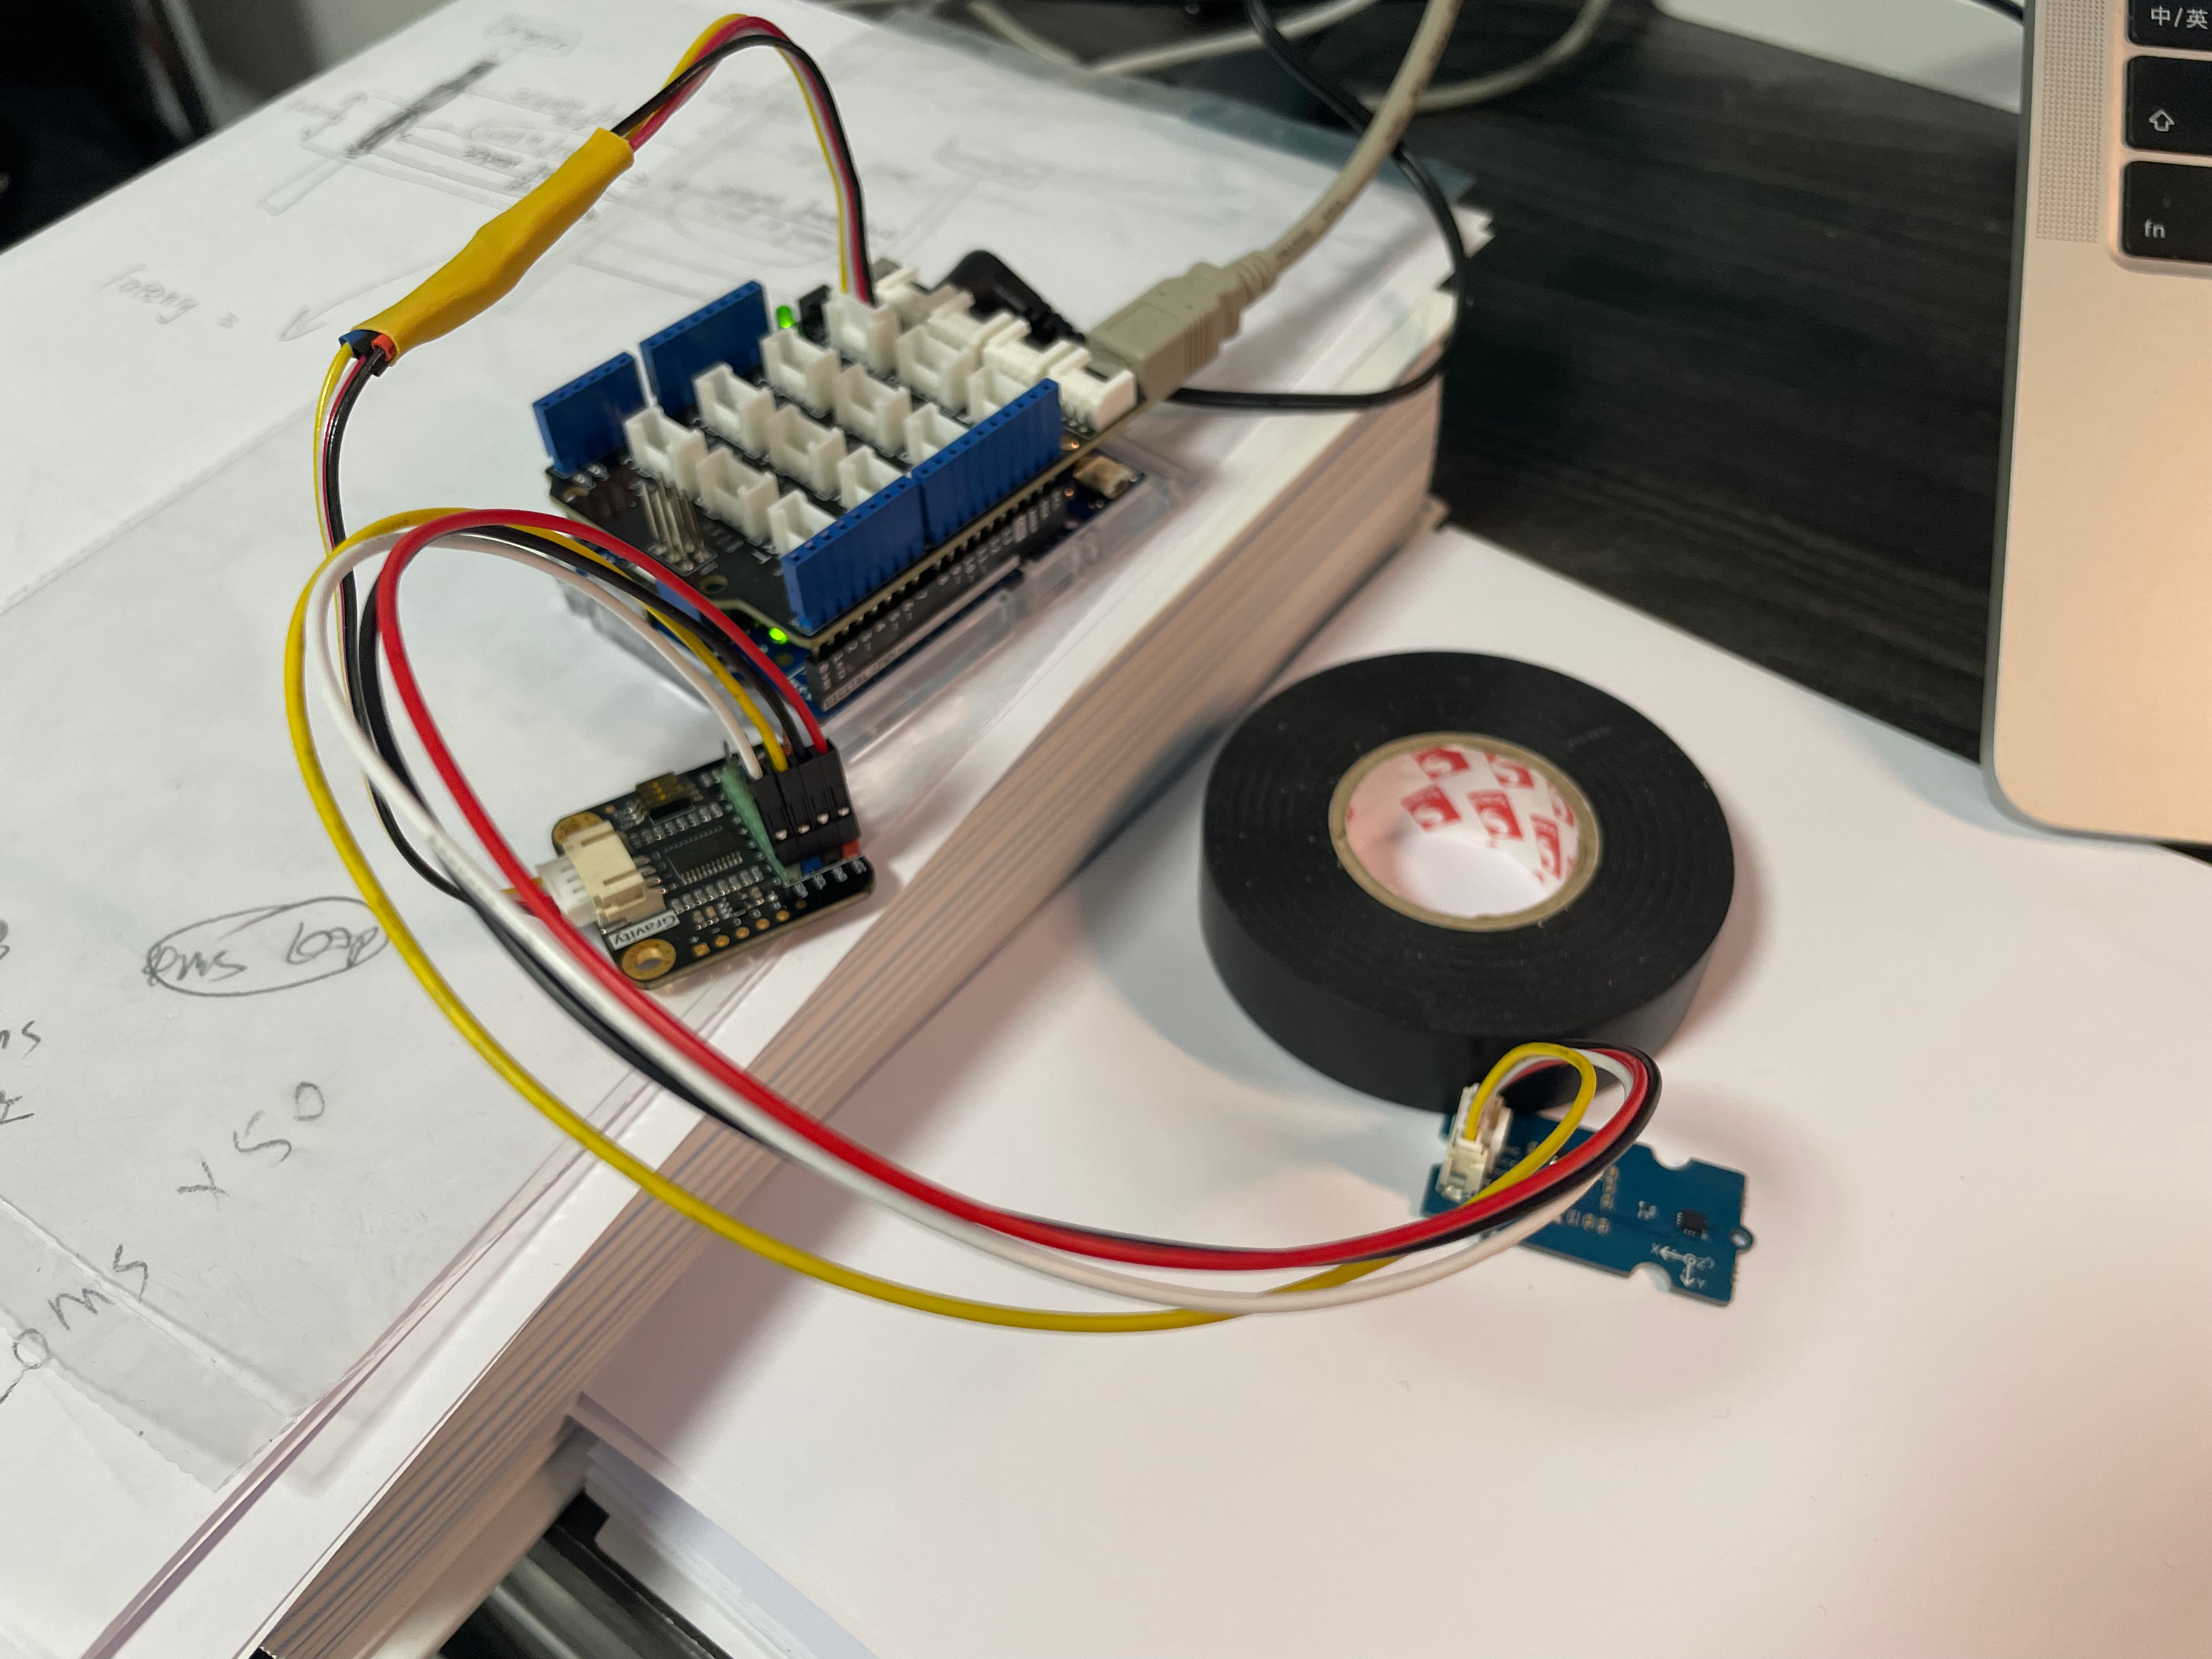
\includegraphics[width=\textwidth]{fileForWriting/original-connection}
		\caption{Original connection using dupont line.}
	\end{subfigure}
	\hfill
	\begin{subfigure}[b]{0.45\textwidth}
		\centering
		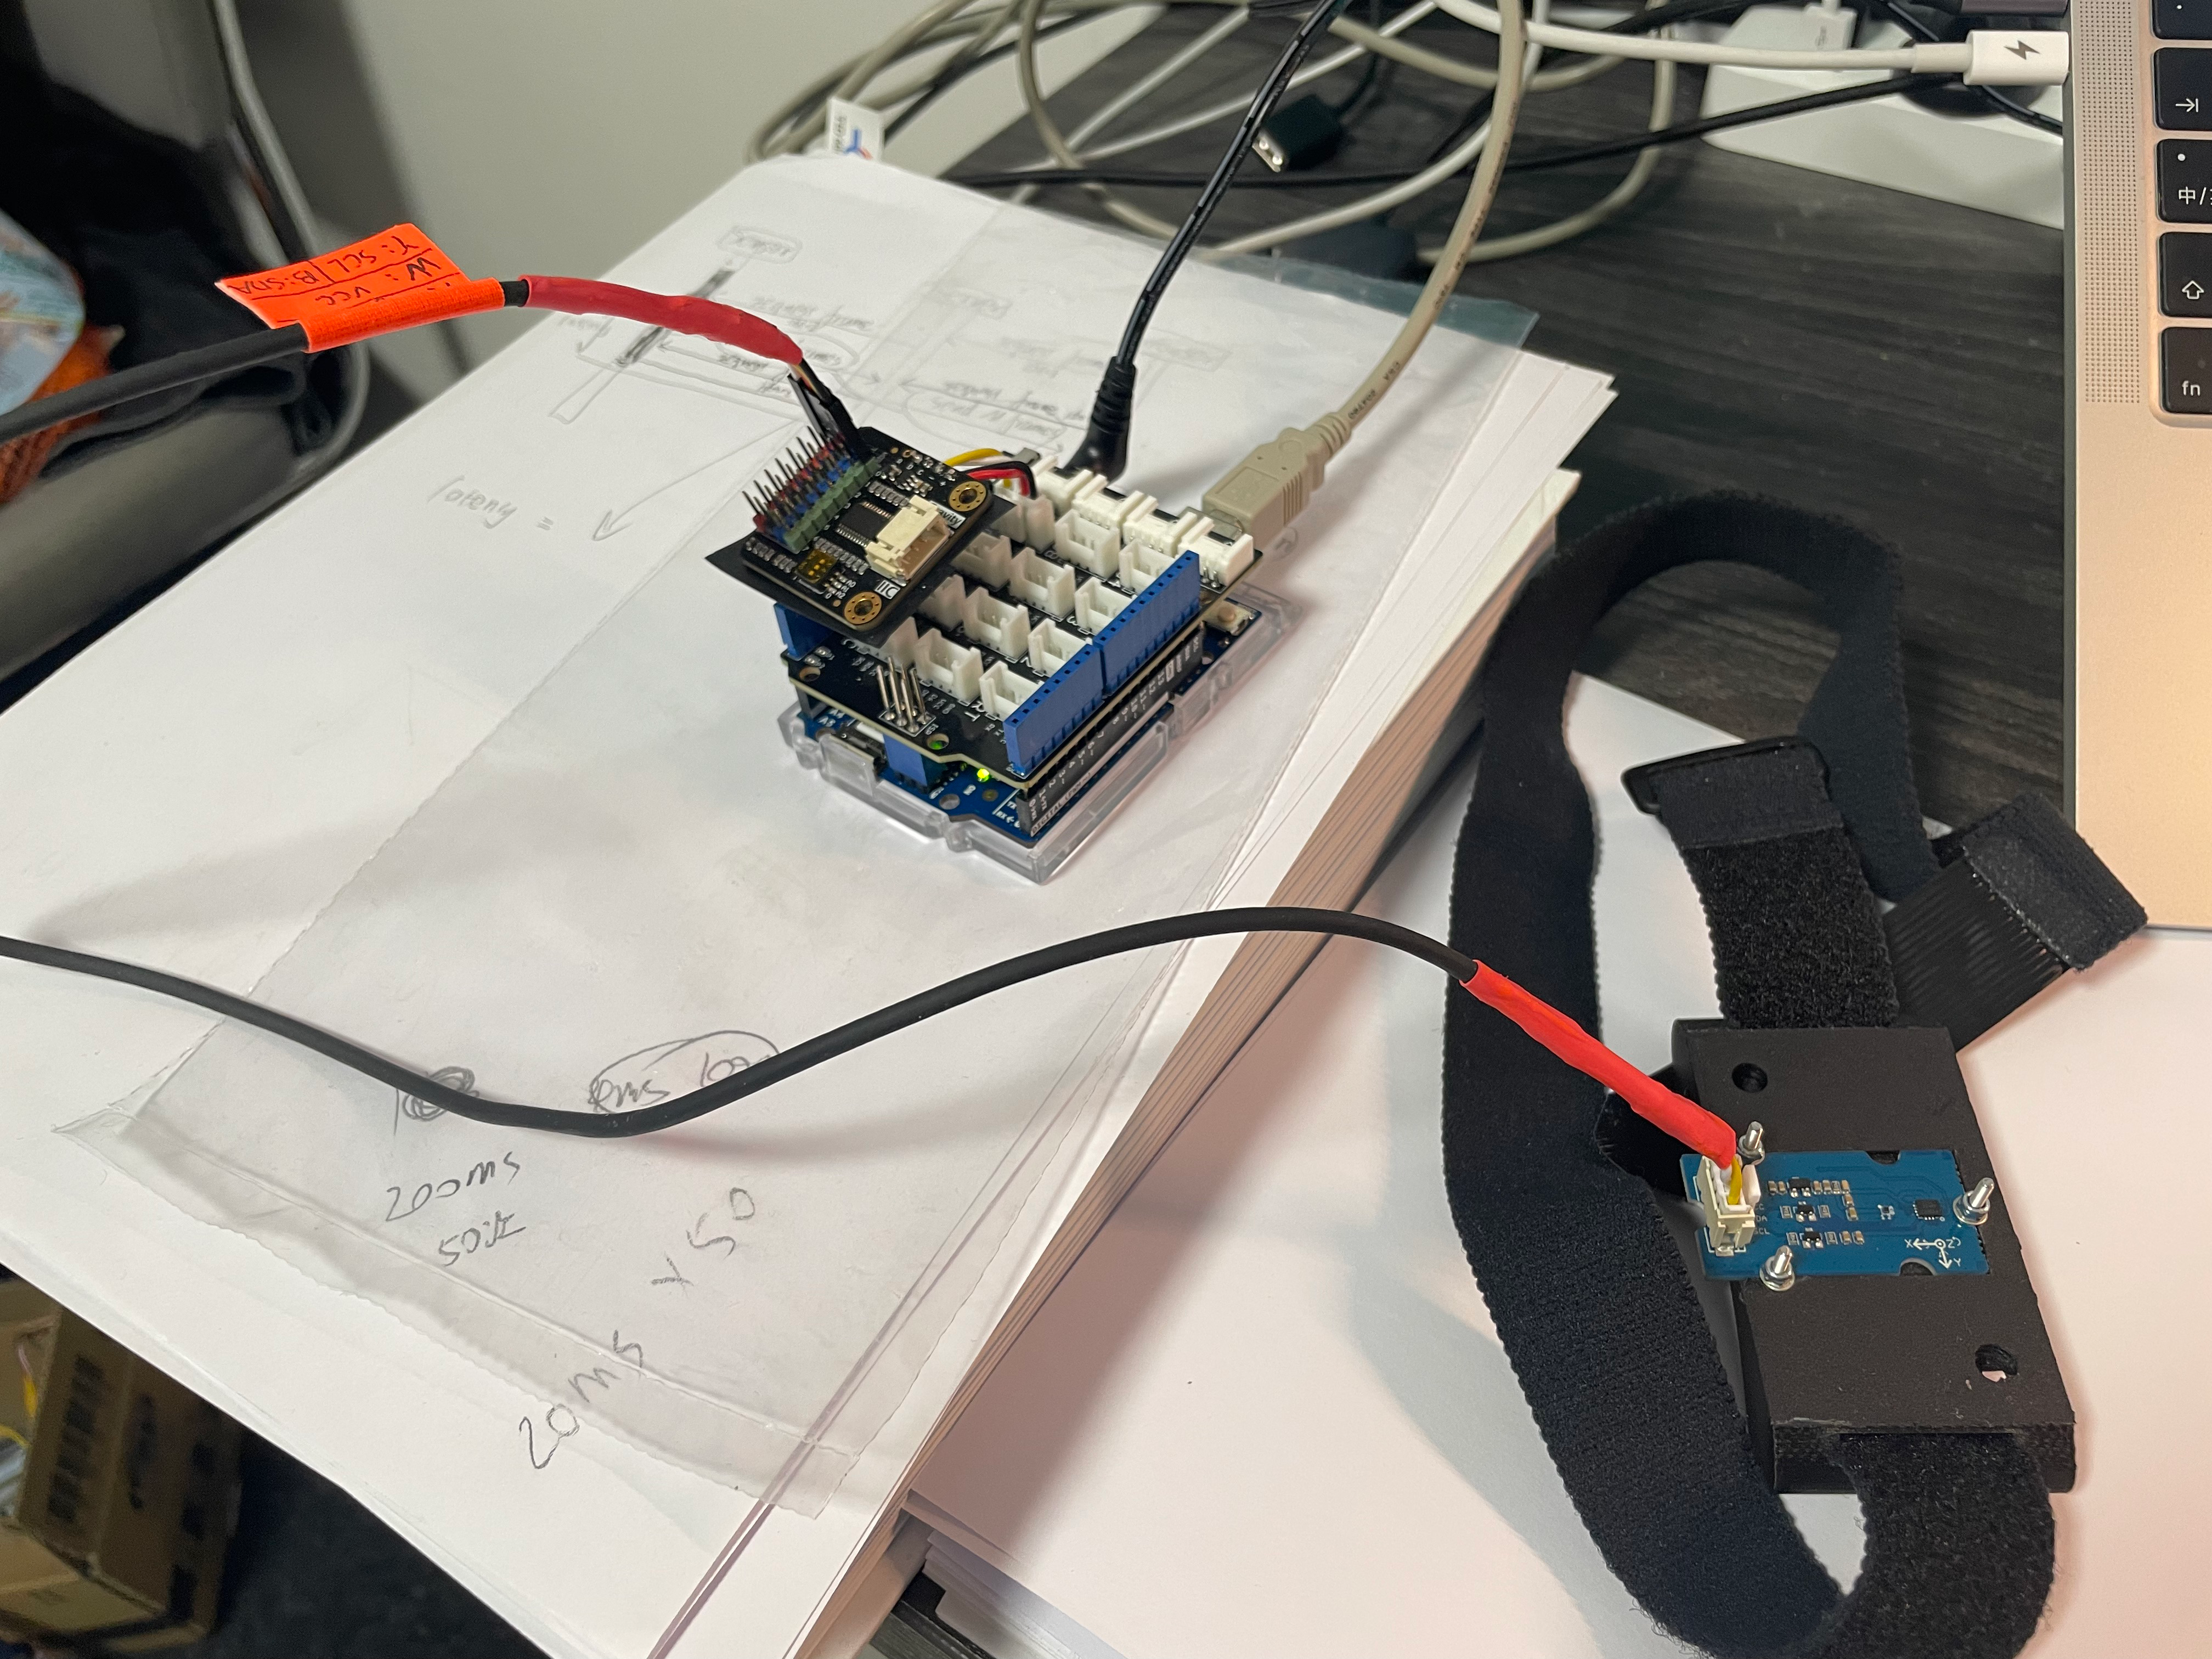
\includegraphics[width=\textwidth]{fileForWriting/improved-connection}
		\caption{Improved connection using screened cable.}
	\end{subfigure}
	\caption[]{Two types of connections to build the external IIC channel.}
	\label{fig:IIC-connections}
\end{figure}

\subsubsection{Remove the ``additional'' IIC channel}
During the following week of testing, the issue did not reoccur.
However, after several accidental drops of the device, the problem resurfaced and the Arduino could not stably send motion data to server.

To solve the issue from root, the ``additional'' IIC channel was physically removed by desoldering two resistors on that channel as Figure~\ref{fig:remove-IIC} may show.
As expected, the Wi-Fi module was indeed functioning well without any interference from external IIC channel.
This success also proved the correctness of previous analysis.


In summary, the Wi-Fi module is very vulnerable to any external interference in its IIC channel.
If affected, it may stop working and throw a ``no socket available'' error.
As the MCU and module use another SPI channel to communicate, we decided to physically remove that IIC channel since this project did not require an IIC functionality of that module.
After the removal, the whole system worked perfectly.
The root of such issue may be the design flaw of Arduino-UNO-Wifi-Rev2, where the MCU, Wi-Fi module, and external IIC devices directly share one IIC channel.
Simultaneously, the Wi-Fi module may require a high level of communication quality.


%-----------This is a FIGURE-----------------------
\begin{figure}[htbp]
	\centering
	\includegraphics[width=0.7\textwidth]{
		fileForWriting/remove IIC}
	\caption{Desoldering two resistors on the ``additional'' IIC channel to completely solve the ``no socket available'' issue.}
	\label{fig:remove-IIC}
\end{figure}
%--------End of this FIGURE -----------







 %list of all materials, methods?
\chapter{Results}

\section{Euler angle}
	just a show, unstable yaw data

\section{Message sending}
	The result of stress test. Latency <=20ms

\section{Displaying engineer}
i.	Flexible to input.

\section{Final Performance}

  %latency & problems occured
\include{discussion-and-conclusions}


%references
\singlespace
\bibliographystyle{IEEEtran}               % References section created automatically
\bibliography{/Users/shenyixiao/Repo/Final-Report/src/MyRefs}                      % The file MyRefs.bib contains the actual bibliography material
\addcontentsline{toc}{chapter}{References} % to add it to the table of contents

%appendix
\newpage
\appendix
\appendixpage
\addappheadtotoc

\chapter{Project Management Forms}
%Appendix A: Attach the project management forms (Role allocation/responsibility matrix, Contribution to project deliverables, Attendance record, Supervisor weekly meeting log) to your project report as an appendix. Other supporting documents you may have used such as personal notes/notebooks/logbooks should not be included in the report.
d
\chapter{A Breakdown of Individual Contributions}
%Appendix B: Include a breakdown of individual contributions to the project, for each and every of the group members. Members of the same group may obtain different marks based on their individual contributions to the project. Please make sure the information provided in this appendix is accurate. Project reports that do not include this appendix will not be marked.
d
\chapter{Datasheets}
%-----------This is a FIGURE-----------------------
\begin{figure}[htbp]
	\centering
	\includegraphics[width=1.1\textwidth]{
		fileForWriting/only two modifiable IIC address}
	\caption[Datasheet of the IMU component]{Partial datasheet of the IMU component. The No.117 register indicates that for one specific compnent, there are at most two selectable IIC addresses to use.}
	\label{fig:limited-IIC-address}
\end{figure}
%--------End of this FIGURE -----------  
\chapter{Codes}



\lstset{language=JavaScript,
	basicstyle=\ttfamily,
	keywordstyle=\color{blue}\ttfamily,
	stringstyle=\color{red}\ttfamily,
	commentstyle=\color{green}\ttfamily,
	morecomment=[l][\color{magenta}]{\#},
	breaklines=true,
	showstringspaces=false}

\lstinputlisting[caption=JavaScript code for flexible-inputting function,label=lst:flexible-input]{codes/flexible-input.js}

\lstinputlisting[caption=JavaScript code for matching and intorpolating data.,label=lst:intorpolation-with-data-matching]{codes/intorpolation-with-data-matching.js}





\end{document}
